\documentclass[11pt]{article}

\usepackage{fullpage}
\usepackage{amsmath, amssymb, bm, cite, epsfig, psfrag}
\usepackage{graphicx}
\usepackage{float}
\usepackage{amsthm}
\usepackage{amsfonts}
\usepackage{listings}
\usepackage{cite}
\usepackage{hyperref}
\usepackage{tikz}
\usepackage{pgfplots}
\pgfplotsset{compat=1.18}
\usepackage{enumerate}
\usepackage{listings}
\usepackage{mathtools}
\lstloadlanguages{Python}
\usetikzlibrary{shapes,arrows}
%\usetikzlibrary{dsp,chains}

\DeclareFixedFont{\ttb}{T1}{txtt}{bx}{n}{9} % for bold
\DeclareFixedFont{\ttm}{T1}{txtt}{m}{n}{9}  % for normal
% Defining colors
\usepackage{color}
\definecolor{deepblue}{rgb}{0,0,0.5}
\definecolor{deepred}{rgb}{0.6,0,0}
\definecolor{deepgreen}{rgb}{0,0.5,0}
\definecolor{backcolour}{rgb}{0.95,0.95,0.92}

%\restylefloat{figure}
%\theoremstyle{plain}      \newtheorem{theorem}{Theorem}
%\theoremstyle{definition} \newtheorem{definition}{Definition}

\def\del{\partial}
\def\ds{\displaystyle}
\def\ts{\textstyle}
\def\beq{\begin{equation}}
\def\eeq{\end{equation}}
\def\beqa{\begin{eqnarray}}
\def\eeqa{\end{eqnarray}}
\def\beqan{\begin{eqnarray*}}
\def\eeqan{\end{eqnarray*}}
\def\nn{\nonumber}
\def\binomial{\mathop{\mathrm{binomial}}}
\def\half{{\ts\frac{1}{2}}}
\def\Half{{\frac{1}{2}}}
\def\N{{\mathbb{N}}}
\def\Z{{\mathbb{Z}}}
\def\Q{{\mathbb{Q}}}
\def\R{{\mathbb{R}}}
\def\C{{\mathbb{C}}}
\def\argmin{\mathop{\mathrm{arg\,min}}}
\def\argmax{\mathop{\mathrm{arg\,max}}}
%\def\span{\mathop{\mathrm{span}}}
\def\diag{\mathop{\mathrm{diag}}}
\def\x{\times}
\def\limn{\lim_{n \rightarrow \infty}}
\def\liminfn{\liminf_{n \rightarrow \infty}}
\def\limsupn{\limsup_{n \rightarrow \infty}}
\def\GV{Guo and Verd{\'u}}
\def\MID{\,|\,}
\def\MIDD{\,;\,}

\newtheorem{proposition}{Proposition}
\newtheorem{definition}{Definition}
\newtheorem{theorem}{Theorem}
\newtheorem{lemma}{Lemma}
\newtheorem{corollary}{Corollary}
\newtheorem{assumption}{Assumption}
\newtheorem{claim}{Claim}
\def\qed{\mbox{} \hfill $\Box$}
\setlength{\unitlength}{1mm}

\def\bhat{\widehat{b}}
\def\ehat{\widehat{e}}
\def\phat{\widehat{p}}
\def\qhat{\widehat{q}}
\def\rhat{\widehat{r}}
\def\shat{\widehat{s}}
\def\uhat{\widehat{u}}
\def\ubar{\overline{u}}
\def\vhat{\widehat{v}}
\def\xhat{\widehat{x}}
\def\xbar{\overline{x}}
\def\zhat{\widehat{z}}
\def\zbar{\overline{z}}
\def\la{\leftarrow}
\def\ra{\rightarrow}
\def\MSE{\mbox{\small \sffamily MSE}}
\def\SNR{\mbox{\small \sffamily SNR}}
\def\SINR{\mbox{\small \sffamily SINR}}
\def\arr{\rightarrow}
\def\Exp{\mathbb{E}}
\def\var{\mbox{var}}
\def\Tr{\mbox{Tr}}
\def\tm1{t\! - \! 1}
\def\tp1{t\! + \! 1}
\def\Tm1{T\! - \! 1}
\def\Tp1{T\! + \! 1}


\def\Xset{{\cal X}}

\newcommand{\one}{\mathbf{1}}
\newcommand{\abf}{\mathbf{a}}
\newcommand{\bbf}{\mathbf{b}}
\newcommand{\dbf}{\mathbf{d}}
\newcommand{\ebf}{\mathbf{e}}
\newcommand{\gbf}{\mathbf{g}}
\newcommand{\hbf}{\mathbf{h}}
\newcommand{\pbf}{\mathbf{p}}
\newcommand{\pbfhat}{\widehat{\mathbf{p}}}
\newcommand{\qbf}{\mathbf{q}}
\newcommand{\qbfhat}{\widehat{\mathbf{q}}}
\newcommand{\rbf}{\mathbf{r}}
\newcommand{\rbfhat}{\widehat{\mathbf{r}}}
\newcommand{\sbf}{\mathbf{s}}
\newcommand{\sbfhat}{\widehat{\mathbf{s}}}
\newcommand{\ubf}{\mathbf{u}}
\newcommand{\ubfhat}{\widehat{\mathbf{u}}}
\newcommand{\utildebf}{\tilde{\mathbf{u}}}
\newcommand{\vbf}{\mathbf{v}}
\newcommand{\vbfhat}{\widehat{\mathbf{v}}}
\newcommand{\wbf}{\mathbf{w}}
\newcommand{\wbfhat}{\widehat{\mathbf{w}}}
\newcommand{\xbf}{\mathbf{x}}
\newcommand{\xbfhat}{\widehat{\mathbf{x}}}
\newcommand{\xbfbar}{\overline{\mathbf{x}}}
\newcommand{\ybf}{\mathbf{y}}
\newcommand{\zbf}{\mathbf{z}}
\newcommand{\zbfbar}{\overline{\mathbf{z}}}
\newcommand{\zbfhat}{\widehat{\mathbf{z}}}
\newcommand{\Ahat}{\widehat{A}}
\newcommand{\Abf}{\mathbf{A}}
\newcommand{\Bbf}{\mathbf{B}}
\newcommand{\Cbf}{\mathbf{C}}
\newcommand{\Bbfhat}{\widehat{\mathbf{B}}}
\newcommand{\Dbf}{\mathbf{D}}
\newcommand{\Gbf}{\mathbf{G}}
\newcommand{\Hbf}{\mathbf{H}}
\newcommand{\Ibf}{\mathbf{I}}
\newcommand{\Kbf}{\mathbf{K}}
\newcommand{\Pbf}{\mathbf{P}}
\newcommand{\Phat}{\widehat{P}}
\newcommand{\Qbf}{\mathbf{Q}}
\newcommand{\Rbf}{\mathbf{R}}
\newcommand{\Rhat}{\widehat{R}}
\newcommand{\Sbf}{\mathbf{S}}
\newcommand{\Ubf}{\mathbf{U}}
\newcommand{\Vbf}{\mathbf{V}}
\newcommand{\Wbf}{\mathbf{W}}
\newcommand{\Xhat}{\widehat{X}}
\newcommand{\Xbf}{\mathbf{X}}
\newcommand{\Ybf}{\mathbf{Y}}
\newcommand{\Zbf}{\mathbf{Z}}
\newcommand{\Zhat}{\widehat{Z}}
\newcommand{\Zbfhat}{\widehat{\mathbf{Z}}}
\def\alphabf{{\boldsymbol \alpha}}
\def\betabf{{\boldsymbol \beta}}
\def\betabfhat{{\widehat{\bm{\beta}}}}
\def\epsilonbf{{\boldsymbol \epsilon}}
\def\mubf{{\boldsymbol \mu}}
\def\lambdabf{{\boldsymbol \lambda}}
\def\etabf{{\boldsymbol \eta}}
\def\xibf{{\boldsymbol \xi}}
\def\taubf{{\boldsymbol \tau}}
\def\sigmahat{{\widehat{\sigma}}}
\def\thetabf{{\bm{\theta}}}
\def\thetabfhat{{\widehat{\bm{\theta}}}}
\def\thetahat{{\widehat{\theta}}}
\def\mubar{\overline{\mu}}
\def\muavg{\mu}
\def\sigbf{\bm{\sigma}}
\def\etal{\emph{et al.}}
\def\Ggothic{\mathfrak{G}}
\def\Pset{{\mathcal P}}
\newcommand{\bigCond}[2]{\bigl({#1} \!\bigm\vert\! {#2} \bigr)}
\newcommand{\BigCond}[2]{\Bigl({#1} \!\Bigm\vert\! {#2} \Bigr)}
\newcommand{\tran}{^{\text{\sf T}}}
\newcommand{\herm}{^{\text{\sf H}}}
\newcommand{\bkt}[1]{{\langle #1 \rangle}}
\def\Norm{{\mathcal N}}
\newcommand{\vmult}{.}
\newcommand{\vdiv}{./}


% Python style for highlighting
\newcommand\pythonstyle{\lstset{
language=Python,
backgroundcolor=\color{backcolour},
commentstyle=\color{deepgreen},
basicstyle=\ttm,
otherkeywords={self},             % Add keywords here
keywordstyle=\ttb\color{deepblue},
emph={MyClass,__init__},          % Custom highlighting
emphstyle=\ttb\color{deepred},    % Custom highlighting style
stringstyle=\color{deepgreen},
%frame=tb,                         % Any extra options here
showstringspaces=false            %
}}

% Python environment
\lstnewenvironment{python}[1][]
{
\pythonstyle
\lstset{#1}
}
{}

% Python for external files
\newcommand\pythonexternal[2][]{{
\pythonstyle
\lstinputlisting[#1]{#2}}}

% Python for inline
\newcommand\pycode[1]{{\pythonstyle\lstinline!#1!}}

\begin{document}

\title{Introduction to Machine Learning\\
Unit 7 Problems:  Gradient Calculations and Nonlinear Optimization}
\author{Prof. Sundeep Rangan}
\date{}

\maketitle

%Submit answers only to problems 1, 2, 3 and 4(b) and (c).  You do not need to answer  4(a).
%But, make sure you know how to do all the problems.
%I looked at the solution, I think the students should be able to do all of them.

\begin{enumerate}

\item \emph{Simple gradient calculation.}  Consider a function,
\[
    J = z_1e^{z_1z_2}, \quad z_1 = a_1w_1w_2, \quad z_2 = a_2w_1 + a_3w_2^2,
\]
\begin{enumerate}[(a)]
\item Compute the partial derivatives, $\partial J/\partial w_j$ for $j=1,2$.
\item Write a python function that, given $\wbf$ and $\abf$
computes $J(\wbf)$ and $\nabla J(\wbf)$.
\end{enumerate}

\textbf{Solution:}
\begin{enumerate}[(a)]
\item Using the chain rule:
$$\frac{\partial J}{\partial w_1} = \frac{\partial J}{\partial z_1}\frac{\partial z_1}{\partial w_1} + \frac{\partial J}{\partial z_2}\frac{\partial z_2}{\partial w_1}$$

First, compute the partial derivatives:
\begin{align}
\frac{\partial J}{\partial z_1} &= e^{z_1z_2} + z_1e^{z_1z_2}z_2 = e^{z_1z_2}(1 + z_1z_2)\\
\frac{\partial J}{\partial z_2} &= z_1e^{z_1z_2}z_1 = z_1^2e^{z_1z_2}\\
\frac{\partial z_1}{\partial w_1} &= a_1w_2\\
\frac{\partial z_1}{\partial w_2} &= a_1w_1\\
\frac{\partial z_2}{\partial w_1} &= a_2\\
\frac{\partial z_2}{\partial w_2} &= 2a_3w_2
\end{align}

Therefore:
$$\frac{\partial J}{\partial w_1} = e^{z_1z_2}(1 + z_1z_2) \cdot a_1w_2 + z_1^2e^{z_1z_2} \cdot a_2 = e^{z_1z_2}[a_1w_2(1 + z_1z_2) + a_2z_1^2]$$

$$\frac{\partial J}{\partial w_2} = e^{z_1z_2}(1 + z_1z_2) \cdot a_1w_1 + z_1^2e^{z_1z_2} \cdot 2a_3w_2 = e^{z_1z_2}[a_1w_1(1 + z_1z_2) + 2a_3w_2z_1^2]$$

\item 
\begin{python}
def Jeval(w, a):
    w1, w2 = w[0], w[1]
    a1, a2, a3 = a[0], a[1], a[2]
    
    # Compute intermediate variables
    z1 = a1 * w1 * w2
    z2 = a2 * w1 + a3 * w2**2
    
    # Compute J
    J = z1 * np.exp(z1 * z2)
    
    # Compute gradients
    exp_term = np.exp(z1 * z2)
    grad_w1 = exp_term * (a1 * w2 * (1 + z1 * z2) + a2 * z1**2)
    grad_w2 = exp_term * (a1 * w1 * (1 + z1 * z2) + 2 * a3 * w2 * z1**2)
    
    return J, np.array([grad_w1, grad_w2])
\end{python}
\end{enumerate}

\item \emph{Gradient with a logarithmic loss.}  Consider the loss function,
\[
    J(\wbf,b) := \sum_{i=1}^N (\log(y_i)-\log(\hat{y}_i))^2,
    \quad \hat{y}_i = \sum_{j=1}^p x_{ij}w_j + b,
\]
This is an MSE loss function, but in log domain.
\begin{enumerate}[(a)]
\item Find the gradient components, $\partial J/\partial w_j$ and $\partial J/\partial b$.
\item Complete the following python function
\begin{python}
    def Jeval(w,b,...):
        ...
        return J, Jgradw, Jgradb
\end{python}
that computes $J$ and $\nabla_w J$ and $\nabla_b J$.
You need to complete the arguments of the function.
To receive full credit, avoid using for loops.
\end{enumerate}

\textbf{Solution:}
\begin{enumerate}[(a)]
\item Let $r_i = \log(y_i) - \log(\hat{y}_i)$. Then $J = \sum_{i=1}^N r_i^2$.

For $\frac{\partial J}{\partial w_j}$:
$$\frac{\partial J}{\partial w_j} = \sum_{i=1}^N 2r_i \frac{\partial r_i}{\partial w_j}$$

Since $r_i = \log(y_i) - \log(\hat{y}_i)$ and $\hat{y}_i = \sum_{k=1}^p x_{ik}w_k + b$:
$$\frac{\partial r_i}{\partial w_j} = -\frac{1}{\hat{y}_i} \frac{\partial \hat{y}_i}{\partial w_j} = -\frac{x_{ij}}{\hat{y}_i}$$

Therefore:
$$\frac{\partial J}{\partial w_j} = \sum_{i=1}^N 2r_i \left(-\frac{x_{ij}}{\hat{y}_i}\right) = -2\sum_{i=1}^N \frac{r_i x_{ij}}{\hat{y}_i}$$

For $\frac{\partial J}{\partial b}$:
$$\frac{\partial J}{\partial b} = \sum_{i=1}^N 2r_i \frac{\partial r_i}{\partial b} = \sum_{i=1}^N 2r_i \left(-\frac{1}{\hat{y}_i}\right) = -2\sum_{i=1}^N \frac{r_i}{\hat{y}_i}$$

\item 
\begin{python}
def Jeval(w, b, X, y):
    # Compute predictions
    yhat = X @ w + b
    
    # Compute residuals in log domain
    r = np.log(y) - np.log(yhat)
    
    # Compute loss
    J = np.sum(r**2)
    
    # Compute gradients
    Jgradw = -2 * np.sum((r / yhat)[:, np.newaxis] * X, axis=0)
    Jgradb = -2 * np.sum(r / yhat)
    
    return J, Jgradw, Jgradb
\end{python}
\end{enumerate}

\item \emph{Gradient with an inverse function.}
Consider the nonlinear least squares fit loss funciton
\[
    J(\wbf) = \sum_{i=1}^n \left[y_i -
        \frac{1}{w_0 + \sum_{j=1}^d w_jx_{ij}}\right]^2.
\]
\begin{enumerate}[(a)]
\item Compute the gradient components, $\partial J/\partial w_j$.
You may want to define the intermediate variable,
\[
    z_i = w_0 + \sum_{j=1}^d w_jx_{ij}.
\]
Also, you can write separate answers for $\partial J/\partial w_0$ and $\partial J/w_j$
for $j = 1,\ldots,d$.

\item Complete the following function to compute the loss and gradient,
\begin{python}
    def Jeval(w,...):
        ...
        return J, Jgrad
\end{python}
For the gradient, you may wish to use the function,
\begin{python}
    Jgrad = np.hstack((Jgrad0, Jgrad1))
\end{python}
to stack two vectors.
\end{enumerate}

\textbf{Solution:}
\begin{enumerate}[(a)]
\item Let $z_i = w_0 + \sum_{j=1}^d w_jx_{ij}$ and $r_i = y_i - \frac{1}{z_i}$.

Then $J = \sum_{i=1}^n r_i^2$.

For $\frac{\partial J}{\partial w_0}$:
$$\frac{\partial J}{\partial w_0} = \sum_{i=1}^n 2r_i \frac{\partial r_i}{\partial w_0}$$

Since $r_i = y_i - \frac{1}{z_i}$ and $\frac{\partial z_i}{\partial w_0} = 1$:
$$\frac{\partial r_i}{\partial w_0} = -\frac{\partial}{\partial w_0}\left(\frac{1}{z_i}\right) = \frac{1}{z_i^2} \frac{\partial z_i}{\partial w_0} = \frac{1}{z_i^2}$$

Therefore:
$$\frac{\partial J}{\partial w_0} = \sum_{i=1}^n 2r_i \frac{1}{z_i^2} = 2\sum_{i=1}^n \frac{r_i}{z_i^2}$$

For $\frac{\partial J}{\partial w_j}$ where $j = 1,\ldots,d$:
$$\frac{\partial J}{\partial w_j} = \sum_{i=1}^n 2r_i \frac{\partial r_i}{\partial w_j}$$

Since $\frac{\partial z_i}{\partial w_j} = x_{ij}$:
$$\frac{\partial r_i}{\partial w_j} = -\frac{\partial}{\partial w_j}\left(\frac{1}{z_i}\right) = \frac{1}{z_i^2} \frac{\partial z_i}{\partial w_j} = \frac{x_{ij}}{z_i^2}$$

Therefore:
$$\frac{\partial J}{\partial w_j} = \sum_{i=1}^n 2r_i \frac{x_{ij}}{z_i^2} = 2\sum_{i=1}^n \frac{r_i x_{ij}}{z_i^2}$$

\item 
\begin{python}
def Jeval(w, X, y):
    w0 = w[0]
    w1 = w[1:]
    
    # Compute z_i = w_0 + sum(w_j * x_{ij})
    z = w0 + X @ w1
    
    # Compute residuals
    r = y - 1/z
    
    # Compute loss
    J = np.sum(r**2)
    
    # Compute gradients
    Jgrad0 = 2 * np.sum(r / z**2)
    Jgrad1 = 2 * np.sum((r / z**2)[:, np.newaxis] * X, axis=0)
    
    # Stack gradients
    Jgrad = np.hstack((Jgrad0, Jgrad1))
    
    return J, Jgrad
\end{python}
\end{enumerate}

\item \emph{Gradient with nonlinear parametrization.}  Given data $(x_i,y_i)$ with
binary class labels $y_i \in \{0,1\}$, consider the
binary cross-entropy loss function,
\[
    J(\abf,\bbf) := \sum_{i=1}^N \log(1+e^{z_i}) - y_iz_i,
    \quad
    z_i = \sum_{j=1}^d a_j e^{-(x_i-b_j)^2/2}.
\]
\begin{enumerate}[(a)]
\item Compute the gradient components, $\partial J/\partial a_j$ and $\partial J/\partial b_j$.

\item Complete the following function to compute the loss and gradient,
\begin{python}
    def Jeval(a,b,...):
        ...
        return J, Jgrada, Jgradb
\end{python}
Avoid for loops to receive full credit.
\end{enumerate}

\textbf{Solution:}
\begin{enumerate}[(a)]
\item Let $J = \sum_{i=1}^N [\log(1+e^{z_i}) - y_iz_i]$ where $z_i = \sum_{j=1}^d a_j e^{-(x_i-b_j)^2/2}$.

For $\frac{\partial J}{\partial a_j}$:
$$\frac{\partial J}{\partial a_j} = \sum_{i=1}^N \left[\frac{e^{z_i}}{1+e^{z_i}} \frac{\partial z_i}{\partial a_j} - y_i \frac{\partial z_i}{\partial a_j}\right]$$

Since $\frac{\partial z_i}{\partial a_j} = e^{-(x_i-b_j)^2/2}$:
$$\frac{\partial J}{\partial a_j} = \sum_{i=1}^N \left[\frac{e^{z_i}}{1+e^{z_i}} - y_i\right] e^{-(x_i-b_j)^2/2}$$

For $\frac{\partial J}{\partial b_j}$:
$$\frac{\partial J}{\partial b_j} = \sum_{i=1}^N \left[\frac{e^{z_i}}{1+e^{z_i}} \frac{\partial z_i}{\partial b_j} - y_i \frac{\partial z_i}{\partial b_j}\right]$$

Since $\frac{\partial z_i}{\partial b_j} = a_j e^{-(x_i-b_j)^2/2} \cdot (x_i - b_j)$:
$$\frac{\partial J}{\partial b_j} = \sum_{i=1}^N \left[\frac{e^{z_i}}{1+e^{z_i}} - y_i\right] a_j e^{-(x_i-b_j)^2/2} (x_i - b_j)$$

\item 
\begin{python}
def Jeval(a, b, x, y):
    # Compute z_i for all i
    # x: (N,), a: (d,), b: (d,)
    # Broadcasting: (N,1) - (1,d) = (N,d)
    diff = x[:, np.newaxis] - b[np.newaxis, :]  # (N,d)
    exp_term = np.exp(-diff**2 / 2)  # (N,d)
    z = np.sum(a * exp_term, axis=1)  # (N,)
    
    # Compute sigmoid and loss
    sigmoid = 1 / (1 + np.exp(-z))  # (N,)
    J = np.sum(np.log(1 + np.exp(z)) - y * z)
    
    # Compute gradients
    residual = sigmoid - y  # (N,)
    
    # Gradient w.r.t. a
    Jgrada = np.sum(residual[:, np.newaxis] * exp_term, axis=0)  # (d,)
    
    # Gradient w.r.t. b  
    Jgradb = np.sum(residual[:, np.newaxis] * a * exp_term * diff, axis=0)  # (d,)
    
    return J, Jgrada, Jgradb
\end{python}
\end{enumerate}

\item \emph{Finding local and global minima}.  Consider the function
\[
    f(x) = \frac{1}{4}x^2 + 1 - \cos(2\pi x).
\]
\begin{enumerate}[(a)]
\item Approximately draw $f(x)$.
\item Write an equation for the gradient descent update to minimize $f(x)$.
\item Using the graph in part (a), where is the global minima of $f(x)$?
\item Using the graph in part (a), find one initial condition where gradient descent
could end up converging to a local minima that is not the global minima.
The local minima do not have a closed form expression, but you should be
able to use the graph in part (a) to ``eyeball" an initial condition close to
a bad local minima.
\end{enumerate}

\textbf{Solution:}
\begin{enumerate}[(a)]
\item The function $f(x) = \frac{1}{4}x^2 + 1 - \cos(2\pi x)$ has:
\begin{itemize}
\item A quadratic term $\frac{1}{4}x^2$ that creates a parabola centered at $x=0$
\item A periodic term $-\cos(2\pi x)$ with period 1 that oscillates between -1 and 1
\item The function will have multiple local minima due to the cosine term
\end{itemize}

\begin{figure}[H]
\centering
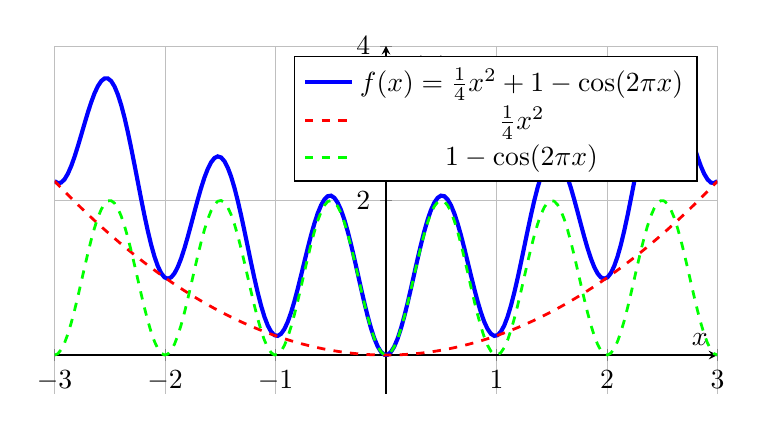
\begin{tikzpicture}
\begin{axis}[
    axis lines = center,
    xlabel = $x$,
    ylabel = $f(x)$,
    xmin = -3, xmax = 3,
    ymin = -0.5, ymax = 4,
    grid = both,
    grid style = {line width=.1pt, draw=gray!10},
    major grid style = {line width=.2pt, draw=gray!50},
    width=10cm,
    height=6cm,
    legend pos = north east,
]
\addplot [
    domain=-3:3,
    samples=200,
    color=blue,
    line width=1.5pt,
] {0.25*x^2 + 1 - cos(2*pi*x*180/pi)};
\addplot [
    domain=-3:3,
    samples=200,
    color=red,
    dashed,
    line width=1pt,
] {0.25*x^2};
\addplot [
    domain=-3:3,
    samples=200,
    color=green,
    dashed,
    line width=1pt,
] {1 - cos(2*pi*x*180/pi)};
\legend{$f(x) = \frac{1}{4}x^2 + 1 - \cos(2\pi x)$, $\frac{1}{4}x^2$, $1 - \cos(2\pi x)$}
\end{axis}
\end{tikzpicture}
\caption{Plot of $f(x) = \frac{1}{4}x^2 + 1 - \cos(2\pi x)$ showing the global minimum at $x=0$ and multiple local minima due to the periodic cosine term.}
\end{figure}

The graph shows a parabola with periodic oscillations. The global minimum is at $x=0$ where $f(0) = 1 - \cos(0) = 0$.

\item The gradient is:
$$f'(x) = \frac{1}{2}x + 2\pi\sin(2\pi x)$$

The gradient descent update is:
$$x^{k+1} = x^k - \alpha f'(x^k) = x^k - \alpha\left(\frac{1}{2}x^k + 2\pi\sin(2\pi x^k)\right)$$

\item The global minimum is at $x = 0$, where $f(0) = 0$.

\item A good initial condition that could lead to a local minimum (not global) would be around $x = \pm 1$ or $x = \pm 2$. For example, starting at $x = 1$:
\begin{itemize}
\item At $x = 1$: $f'(1) = \frac{1}{2} + 2\pi\sin(2\pi) = \frac{1}{2} > 0$
\item The gradient is positive, so gradient descent will move left
\item It could converge to a local minimum around $x \approx 0.5$ or $x \approx -0.5$
\end{itemize}

Another example: starting at $x = 2$:
\begin{itemize}
\item At $x = 2$: $f'(2) = 1 + 2\pi\sin(4\pi) = 1 > 0$  
\item The gradient is positive, so gradient descent will move left
\item It could converge to a local minimum around $x \approx 1.5$ or $x \approx 0.5$
\end{itemize}
\end{enumerate}


\item In this problem, we will see why gradient descent can often exhibit
very slow convergence, even on apparently simple functions.
Consider the objective function,
\[
    J(\wbf) = \frac{1}{2}b_1w_1^2 + \frac{1}{2}b_2w_2^2,
\]
defined on a vector $\wbf=(w_1,w_2)$ with constants $b_2 > b_1 > 0$.
\begin{enumerate}[(a)]
  \item What is the gradient $\nabla J(\wbf)$?
  \item What is the minimum $\wbf^* = \argmin_{\wbf} J(\wbf)$?
  \item Part (b) shows that we can minimize $J(\wbf)$ easily by hand.
  But, suppose we tried to minimize it via gradient descent.
  Show that the gradient descent update of $\wbf$ with a step-size $\alpha$
has the form,
\[
    w_1^{k+1} = \rho_1 w_1^k, \quad w_2^{k+1} = \rho_2 w_2^k,
\]
for some constants $\rho_i$, $i=1,2$.  Write $\rho_i$ in terms of
$b_i$ and the step-size $\alpha$.
  \item For what values $\alpha$ will gradient descent converge to the minimum? That is, what step sizes guarantee that $\wbf^k \arr \wbf^*$.

\item Take $\alpha = 2/(b_1+b_2)$.  It can be shown that this choice of $\alpha$ results in the fastest convergence.  You do not need to show this.
But, show that with this selection of $\alpha$,
\[
    \|\wbf^k\| = C^k \|\wbf^0\|, \quad C = \frac{\kappa-1}{\kappa+1 }, \quad
    \kappa = \frac{b_2}{b_1}.
\]
The term $\kappa$ is called the \emph{condition number}.  The above calculation
shows that when $\kappa$ is very large, $C \approx 1$ and the convergence
of gradient descent is slow.  In general, gradient descent performs poorly
when the problems are ill-conditioned like this.
\end{enumerate}

\textbf{Solution:}
\begin{enumerate}[(a)]
\item The gradient is:
$$\nabla J(\wbf) = \begin{bmatrix} b_1 w_1 \\ b_2 w_2 \end{bmatrix}$$

\item The minimum occurs where the gradient is zero:
$$\nabla J(\wbf^*) = \begin{bmatrix} b_1 w_1^* \\ b_2 w_2^* \end{bmatrix} = \begin{bmatrix} 0 \\ 0 \end{bmatrix}$$

Therefore $\wbf^* = (0, 0)$.

\item The gradient descent update is:
$$\wbf^{k+1} = \wbf^k - \alpha \nabla J(\wbf^k) = \wbf^k - \alpha \begin{bmatrix} b_1 w_1^k \\ b_2 w_2^k \end{bmatrix}$$

This gives:
$$w_1^{k+1} = w_1^k - \alpha b_1 w_1^k = (1 - \alpha b_1) w_1^k = \rho_1 w_1^k$$
$$w_2^{k+1} = w_2^k - \alpha b_2 w_2^k = (1 - \alpha b_2) w_2^k = \rho_2 w_2^k$$

where $\rho_1 = 1 - \alpha b_1$ and $\rho_2 = 1 - \alpha b_2$.

\item For convergence, we need $|\rho_i| < 1$ for $i = 1,2$.

For $\rho_1 = 1 - \alpha b_1$: we need $-1 < 1 - \alpha b_1 < 1$, which gives $0 < \alpha < \frac{2}{b_1}$.

For $\rho_2 = 1 - \alpha b_2$: we need $-1 < 1 - \alpha b_2 < 1$, which gives $0 < \alpha < \frac{2}{b_2}$.

Since $b_2 > b_1$, the more restrictive condition is $\alpha < \frac{2}{b_2}$.

Therefore, gradient descent converges when $0 < \alpha < \frac{2}{b_2}$.

\item With $\alpha = \frac{2}{b_1 + b_2}$:

$$\rho_1 = 1 - \frac{2b_1}{b_1 + b_2} = \frac{b_1 + b_2 - 2b_1}{b_1 + b_2} = \frac{b_2 - b_1}{b_1 + b_2}$$

$$\rho_2 = 1 - \frac{2b_2}{b_1 + b_2} = \frac{b_1 + b_2 - 2b_2}{b_1 + b_2} = \frac{b_1 - b_2}{b_1 + b_2} = -\frac{b_2 - b_1}{b_1 + b_2}$$

Since $b_2 > b_1$, we have $\rho_1 = \frac{b_2 - b_1}{b_1 + b_2}$ and $\rho_2 = -\frac{b_2 - b_1}{b_1 + b_2}$.

The convergence rate is determined by the larger of $|\rho_1|$ and $|\rho_2|$, which is:
$$C = \frac{b_2 - b_1}{b_1 + b_2} = \frac{b_2/b_1 - 1}{b_2/b_1 + 1} = \frac{\kappa - 1}{\kappa + 1}$$

where $\kappa = \frac{b_2}{b_1}$ is the condition number.

The norm decreases as:
$$\|\wbf^k\| = C^k \|\wbf^0\|$$

When $\kappa$ is very large (ill-conditioned), $C \approx 1$ and convergence is slow.
\end{enumerate}

\item \emph{Matrix minimization}.  Consider the problem of finding a matrix
$\Pbf \in \R^{m \x m}$ to minimize the loss function,
\[
    J(\Pbf) = \sum_{i=1}^n \left[ \frac{z_i}{y_i} - \ln(z_i) \right],
    \quad
    z_i = \xbf_i\tran \Pbf \xbf_i.
\]
The problem arises in wireless communications where an $m$-antenna receiver wishes
to estimate a spatial covariance matrix $\Pbf$ from $n$ power measurements.
In this setting, $y_i > 0$ is the $i$-th receive power measurement and $\xbf_i$
is the beamforming direction for that measurement.  In reality, the quantities
would be complex, but for simplicity we will just look at the real-valued case.
See the following article for more details:
\begin{quote}
  Eliasi, Parisa A., Sundeep Rangan, and Theodore S. Rappaport. ``Low-rank spatial channel estimation for millimeter wave cellular systems," \emph{IEEE Transactions on Wireless Communications} 16.5 (2017): 2748-2759.
\end{quote}
\begin{enumerate}[(a)]
\item What is the gradient $\nabla_{\Pbf} z_i$?

\item What is the gradient $\nabla_{\Pbf} J(\Pbf)$?

\item Write a few lines of python code to evaluate $J(\Pbf)$ and
$\nabla_{\Pbf} J(\Pbf)$ given data $\xbf_i$ and $y_i$.  You can use a for loop.

\item See if you can rewrite (c) without a for loop.  You will need Python broadcasting.
\end{enumerate}

\textbf{Solution:}
\begin{enumerate}[(a)]
\item For $z_i = \xbf_i^T \Pbf \xbf_i$, we have:
$$\nabla_{\Pbf} z_i = \xbf_i \xbf_i^T$$

This can be derived using the matrix derivative formula $\frac{\partial}{\partial \Pbf}(\xbf^T \Pbf \xbf) = \xbf \xbf^T$.

\item The gradient of $J(\Pbf)$ is:
$$\nabla_{\Pbf} J(\Pbf) = \sum_{i=1}^n \left[\frac{1}{y_i} - \frac{1}{z_i}\right] \nabla_{\Pbf} z_i = \sum_{i=1}^n \left[\frac{1}{y_i} - \frac{1}{z_i}\right] \xbf_i \xbf_i^T$$

\item 
\begin{python}
def Jeval(P, X, y):
    n, m = X.shape
    J = 0
    grad_P = np.zeros((m, m))
    
    for i in range(n):
        z_i = X[i] @ P @ X[i]
        J += z_i / y[i] - np.log(z_i)
        grad_P += (1/y[i] - 1/z_i) * np.outer(X[i], X[i])
    
    return J, grad_P
\end{python}

\item 
\begin{python}
def Jeval_vectorized(P, X, y):
    # X: (n, m), P: (m, m), y: (n,)
    z = np.sum(X @ P * X, axis=1)  # (n,) - element-wise multiplication
    J = np.sum(z / y - np.log(z))
    
    # Compute gradients using broadcasting
    coeffs = (1/y - 1/z)[:, np.newaxis, np.newaxis]  # (n, 1, 1)
    X_outer = X[:, :, np.newaxis] * X[:, np.newaxis, :]  # (n, m, m)
    grad_P = np.sum(coeffs * X_outer, axis=0)  # (m, m)
    
    return J, grad_P
\end{python}
\end{enumerate}

\item \emph{Nested optimization}.  Suppose we are given a loss function
$J(\wbf_1,\wbf_2)$ with two parameter vectors $\wbf_1$ and $\wbf_2$.
In some cases, it is easy to minimize over one of the sets of parameters, say
$\wbf_2$, while holding the other parameter vector (say, $\wbf_1$) constant.
In this case, one could perform the following \emph{nested} minimization:
Define
\[
    J_1(\wbf_1) := \min_{\wbf_2} J(\wbf_1,\wbf_2), \quad
    \wbfhat_2(\wbf_1) := \argmin_{\wbf_2} J(\wbf_1,\wbf_2),
\]
which represent the minimum and argument of the loss function over $\wbf_2$
holding $\wbf_1$ constant.   Then,
\[
    \wbfhat_1 = \argmin_{\wbf_1} J_1(\wbf_1) = \argmin_{\wbf_1} \min_{\wbf_2}
    J(\wbf_1,\wbf_2).
\]
Hence, we can find the optimal $\wbf_1$ by minimizing $J_1(\wbf_1)$
instead of minimizing $J(\wbf_1,\wbf_2)$ over $\wbf_1$ and $\wbf_2$.
\begin{enumerate}[(a)]
\item Show that the gradient of $J_1(\wbf_1)$ is given by
\[
    \nabla_{\wbf_1} J_1(\wbf_1) = \left. \nabla_{\wbf_1} J(\wbf_1,\wbf_2)\right|_{\wbf_2=\wbfhat_2}.
\]
Thus, given $\wbf_1$, we can evaluate the gradient from (i) solve the minimization
$\wbfhat_2:= \argmin_{\wbf_2} J(\wbf_1,\wbf_2)$; and (ii) take the gradient
$\nabla_{\wbf_1} J(\wbf_1,\wbf_2)$ and evaluate at $\wbf_2 = \wbfhat_2$.

\item Suppose we want to minimize a nonlinear least squares,
\[
    J(\abf,\bbf) := \sum_{i=1}^n \left( y_i -
        \sum_{j=1}^d b_j e^{-a_jx_i} \right)^2,
\]
over two parameters $\abf$ and $\bbf$.  Given parameters $\abf$,
describe how we can minimize over $\bbf$.  That is, how can we compute,
\[
    \hat{\bbf} := \argmin_{\bbf} J(\abf,\bbf).
\]

\item In the above example, how would we compute the gradients,
\[
    \nabla_\abf J(\abf,\bbf).
\]

\end{enumerate}

\textbf{Solution:}
\begin{enumerate}[(a)]
\item By definition, $J_1(\wbf_1) = J(\wbf_1, \wbfhat_2(\wbf_1))$ where $\wbfhat_2(\wbf_1) = \argmin_{\wbf_2} J(\wbf_1,\wbf_2)$.

Using the chain rule:
$$\nabla_{\wbf_1} J_1(\wbf_1) = \nabla_{\wbf_1} J(\wbf_1, \wbfhat_2(\wbf_1)) + \nabla_{\wbf_2} J(\wbf_1, \wbfhat_2(\wbf_1)) \frac{\partial \wbfhat_2}{\partial \wbf_1}$$

However, since $\wbfhat_2(\wbf_1)$ minimizes $J(\wbf_1, \wbf_2)$ over $\wbf_2$, we have:
$$\nabla_{\wbf_2} J(\wbf_1, \wbfhat_2(\wbf_1)) = 0$$

Therefore:
$$\nabla_{\wbf_1} J_1(\wbf_1) = \nabla_{\wbf_1} J(\wbf_1, \wbfhat_2(\wbf_1))$$

This is the \emph{envelope theorem} - the gradient of the optimal value function equals the gradient of the original function with respect to the remaining variables, evaluated at the optimal solution.

\item Given $\abf$, the problem becomes:
$$\hat{\bbf} = \argmin_{\bbf} \sum_{i=1}^n \left( y_i - \sum_{j=1}^d b_j e^{-a_jx_i} \right)^2$$

This is a linear least squares problem in $\bbf$. Let:
$$A_{ij} = e^{-a_jx_i}, \quad \bbf = \begin{bmatrix} b_1 \\ \vdots \\ b_d \end{bmatrix}, \quad \ybf = \begin{bmatrix} y_1 \\ \vdots \\ y_n \end{bmatrix}$$

Then the problem becomes:
$$\hat{\bbf} = \argmin_{\bbf} \|\ybf - A\bbf\|^2$$

The solution is:
$$\hat{\bbf} = (A^T A)^{-1} A^T \ybf$$

\item To compute $\nabla_\abf J(\abf,\bbf)$, we use the envelope theorem from part (a):

$$\nabla_\abf J(\abf,\bbf) = \left. \nabla_\abf J(\abf,\bbf) \right|_{\bbf = \hat{\bbf}(\abf)}$$

where $\hat{\bbf}(\abf)$ is the optimal $\bbf$ for given $\abf$.

The gradient with respect to $\abf$ is:
$$\frac{\partial J}{\partial a_j} = \sum_{i=1}^n 2\left( y_i - \sum_{k=1}^d b_k e^{-a_kx_i} \right) \cdot b_j x_i e^{-a_jx_i}$$

Evaluated at $\bbf = \hat{\bbf}(\abf)$:
$$\nabla_\abf J(\abf,\bbf) = \sum_{i=1}^n 2\left( y_i - \sum_{k=1}^d \hat{b}_k e^{-a_kx_i} \right) \cdot \hat{b}_j x_i e^{-a_jx_i}$$

This gives us the gradient for optimizing $\abf$ using nested optimization.
\end{enumerate}

\end{enumerate}
\end{document}
